\documentclass[a4paper]{article}
\usepackage[utf8]{inputenc}
\usepackage{graphicx}
\usepackage{multirow}
\usepackage{fancyhdr}
\usepackage{hyperref}
\pagestyle{fancy}
\begin{document}
\begin{tabular}{p{7cm}r}
\textbf{Michał Radmacher}&\multirow{10}{*}{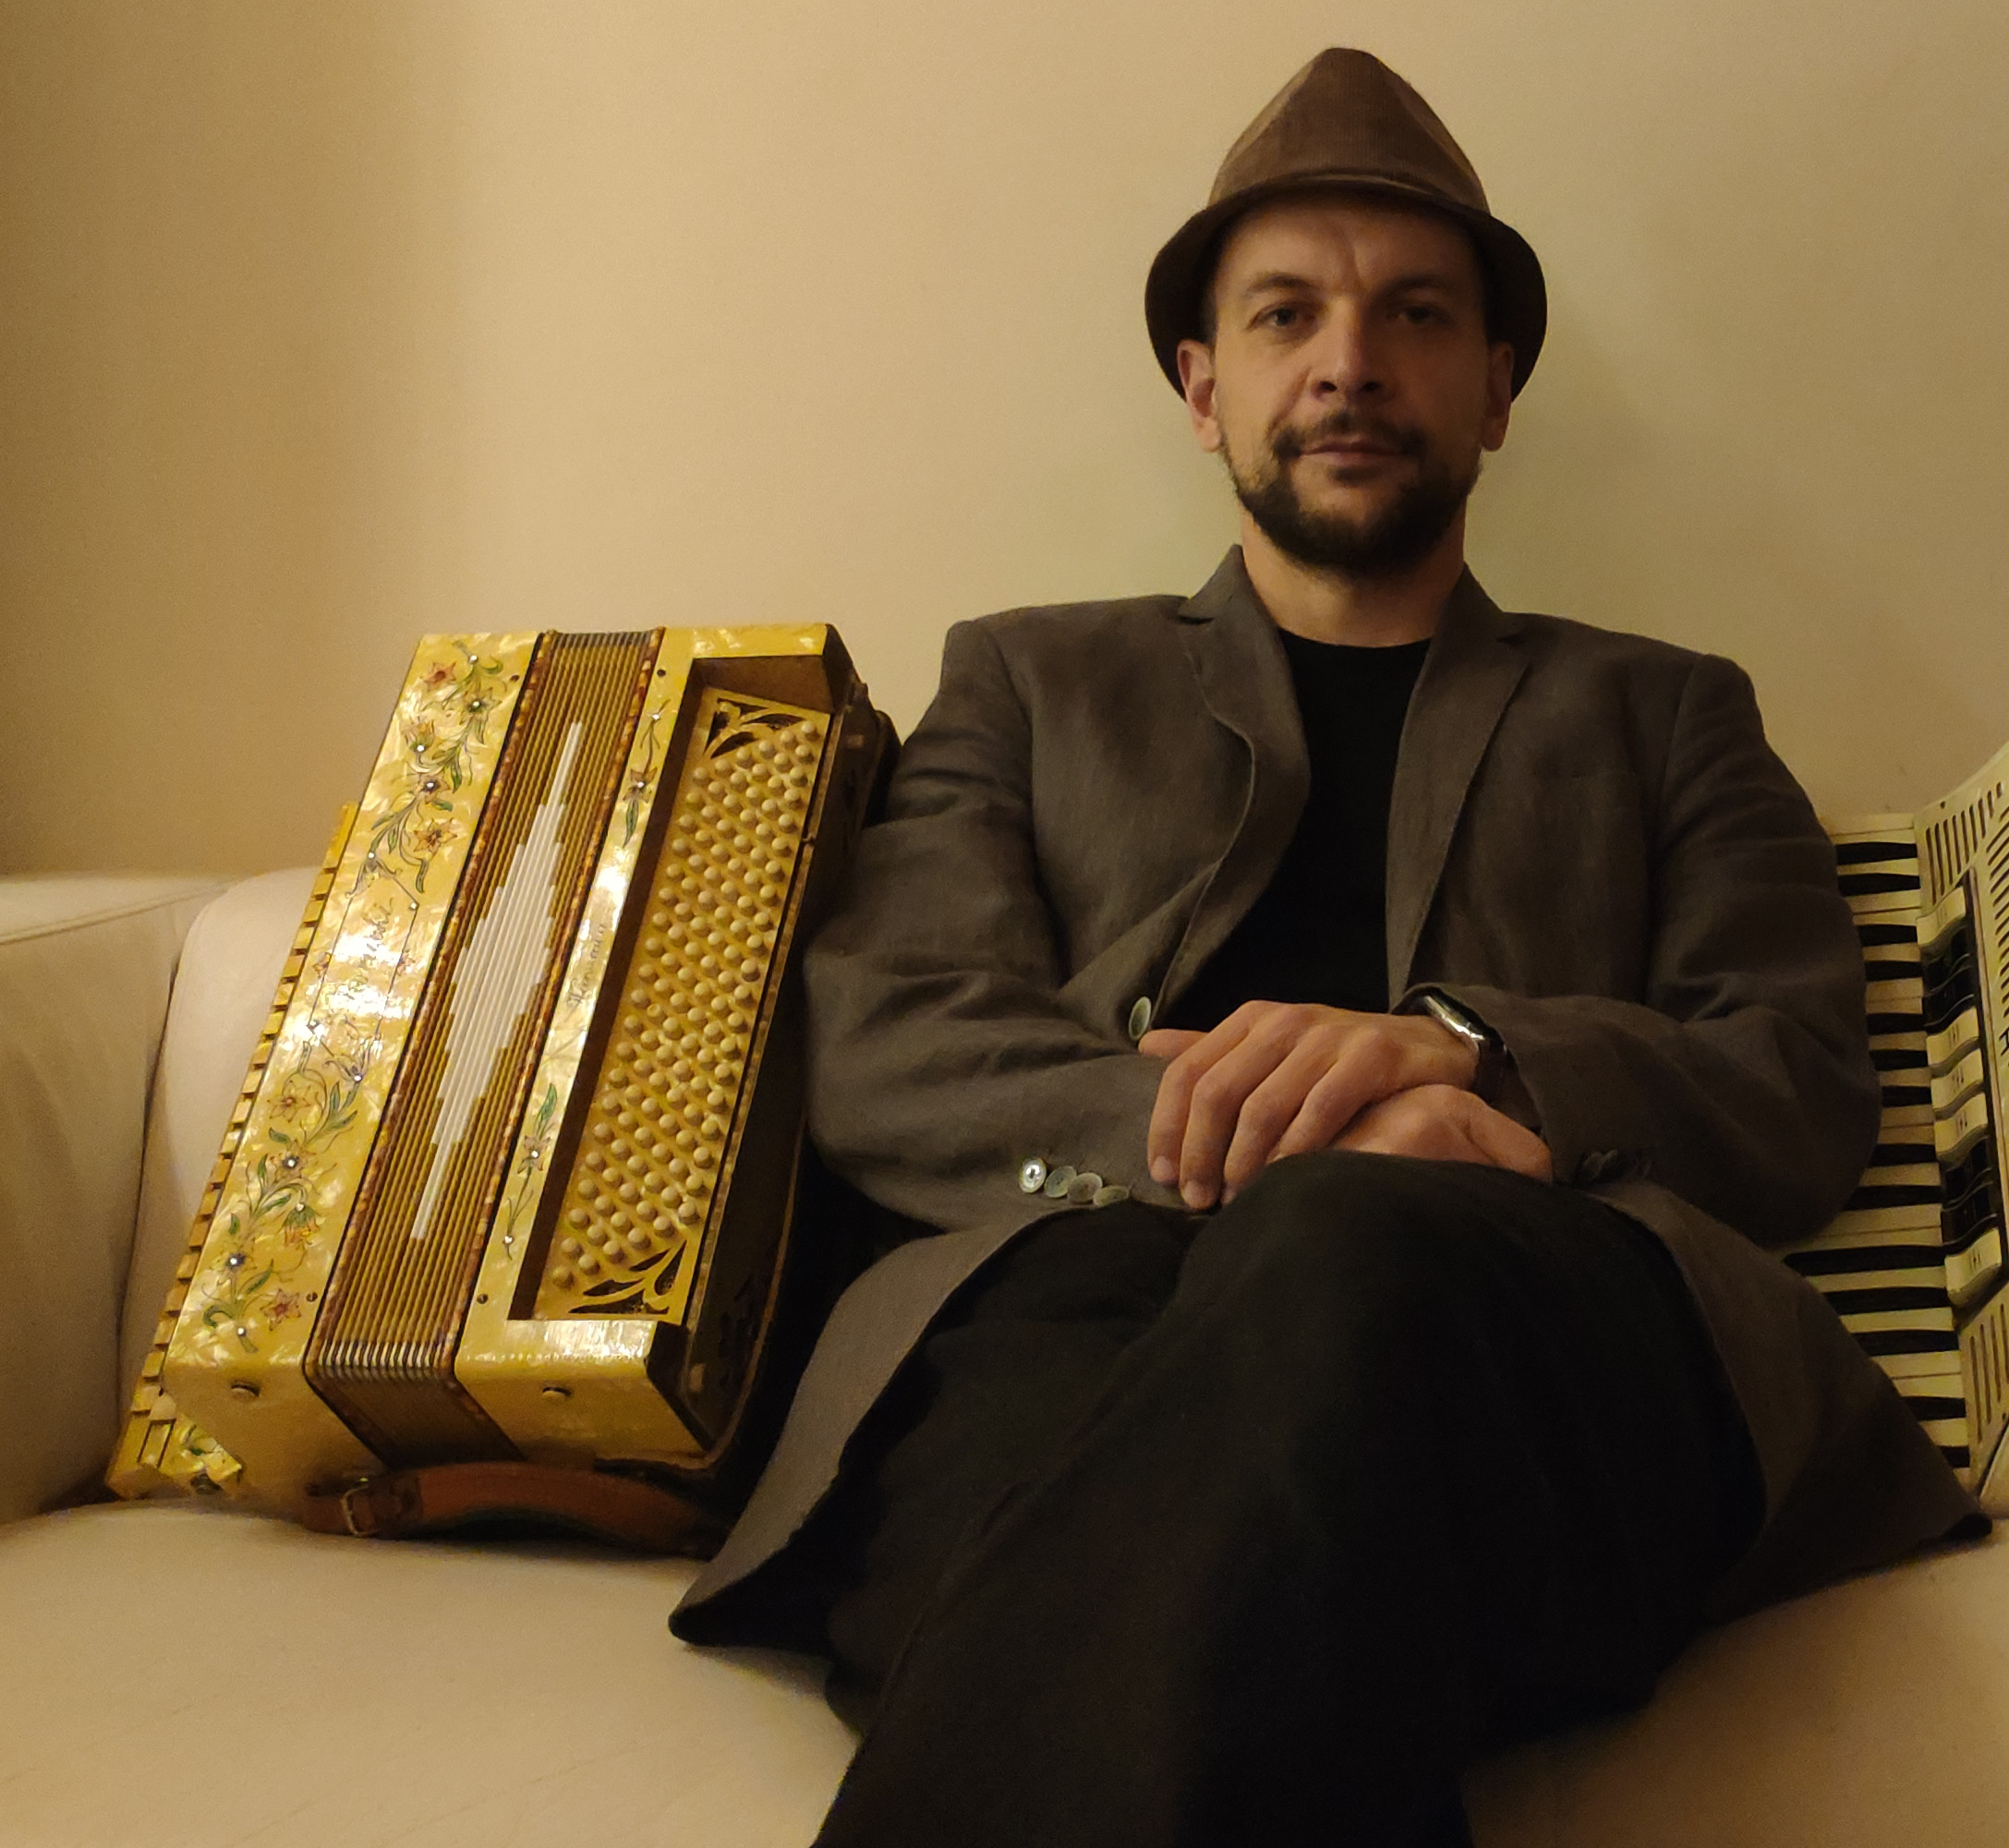
\includegraphics[width=40mm]{mr.jpg}}\\
&\\
+48 662 974 971&\\
michal@radmacher.pl&\\
\href{https://github.com/mradmacher/}{GitHub}\\
&\\
&\\
I like hacking around interesting projects with interesting people.
&\\
&
\end{tabular}

\subsection*{\center{WORK EXPERIENCE}}

\begin{itemize}
  \item
  since 04.2024,
  Zendesk
  \begin{itemize}
    \item
      touching authentication related stuff
    \item
      \textbf{Ruby}
  \end{itemize}
  \item
  03.2014-02.2024,
  CipherHealth
  \begin{itemize}
    \item
      \textbf{healthcare} system for patient engagement, education and screening
    \item
      developing and maintaining key products, integrations, \textbf{automation of communication} with patients
    \item
      \textbf{Ruby}, MongoDB, PostgreSQL, Twilio, Cloud technologies
  \end{itemize}
  \item
    09.2012-02.2014,
    Polcode
    \begin{itemize}
      \item
        designing and developing web applications with direct cooperation with \textbf{international customers}
      \item
        \textbf{Ruby on Rails}, PostgreSQL, JavaScript, HTML, CSS
    \end{itemize}
  \item
    02.2010-08.2012,
    Softelnet
    \begin{itemize}
      \item
        maintaining and developing an inventory system
        for one of the leading Polish \textbf{telecom} operators
      \item
        \textbf{PowerBuilder}, \textbf{PL/SQL}, SQL
    \end{itemize}
  \item
    11.2008-01.2010,
    Seihosoft
    \begin{itemize}
      \item
        designing and implementation of \textbf{distributed computer system}
        for a chain of stores
      \item
        \textbf{Java}, JMS, Hibernate
    \end{itemize}
  \item
    Personal projects
    \begin{itemize}
      \item
        \href{https://github.com/mradmacher/paleolog}{PaleoLog} - a web app for geologists for samples counting, analysis and results sharing.
      \item
        I play music. I've created websites for my bands: \href{https://etnorozrabiaka.art}{etnorozrabiaka.art}, \href{https://iglika.eu}{iglika.eu}, \href{https://czarnymotyl.art}{czarnymotyl.art} \href{https://balkanartz.eu}{balkanartz.eu}, \href{https://karoryfer.com}{karoryfer.com}.
      \item
        Some \href{https://rubygems.org/profiles/mradmacher}{gems} and \href{https://github.com/mradmacher?tab=repositories}{other stuff}.
    \end{itemize}
\end{itemize}

\subsection*{\center{SKILLS}}
\begin{itemize}
\item
  \textbf{Ruby}, JavaScript, Go
\item
  C, Zig, Elixir - I'll get there
\item
  PostgreSQL, MongoDB
\item
  Linux
\item
  Git
\item
  Vim
\end{itemize}

\subsection*{\center{LANGUAGES}}
\begin{itemize}
\item
  \textbf{Polish} --- native
\item
  \textbf{English}, Spanish, Russian, Bulgarian --- communicative
\item
  Ukrainian, Greek --- working on it
\end{itemize}

\subsection*{\center{EDUCATION}}
\begin{itemize}
  \item
    10.2005-05.2009 \textbf{Engineer}, School of Banking and Management in Krakow, IT

  \item
    10.2001-05.2005 Incomplete Higher Education,
    \textbf{Jagielonian University in Krakow, Mathematics}

  \item
    1998-2004 \textbf{Musician},
    Second level Musical State School of Władysław Żeleński in Krakow
\end{itemize}

\subsection*{\center{OTHER INTERESTS}}
\begin{itemize}
\item
	I play clarinet, accordion and some other instruments.
\item
  I learn human and computer languages.
\item
  I practise karate.
\end{itemize}
\end{document}
